% Created 2015-07-08 Wed 19:13
\documentclass[bigger]{beamer}
\usepackage[utf8]{inputenc}
\usepackage[T1]{fontenc}
\usepackage{fixltx2e}
\usepackage{graphicx}
\usepackage{longtable}
\usepackage{float}
\usepackage{wrapfig}
\usepackage{rotating}
\usepackage[normalem]{ulem}
\usepackage{amsmath}
\usepackage{textcomp}
\usepackage{marvosym}
\usepackage{wasysym}
\usepackage{amssymb}
\usepackage{hyperref}
\tolerance=1000
\mode<beamer>{\usetheme{CambridgeUS}\usecolortheme{whale}\usecolortheme{wolverine}}
\begin{center}

\includegraphics[height=50pt]{fig/LNCC_azul.jpg} \hspace*{-30pt}
\end{center}
\vspace*{-45pt}
\author{Martha Hilda Timoteo Sanchez, Rafael Lemes Beirigo}
\date{\today}
\title{Análise de complexidade para Listas Ligadas Simples e Duplas}
\hypersetup{
  pdfkeywords={algoritmos, complexidade, listas ligadas, listas duplamente encadeadas},
  pdfsubject={Análise de complexidade para Listas Ligadas Simples e Duplas},
  pdfcreator={Emacs 24.5.1 (Org mode 8.2.10)}}
\begin{document}

\maketitle
\tableofcontents


\section{Lista Ligada Simples}
\label{sec-1}
\subsection{Lista Ligada Simples}
\label{sec-1-1}
\subsubsection{Lista Ligada Simples}
\label{sec-1-1-1}
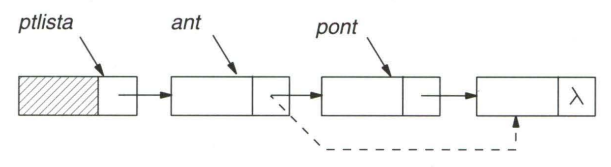
\includegraphics[width=.9\linewidth]{fig/listasimple.png}
\begin{itemize}
\item um ponteiro para o posterior
\item percurso unidirecional
\end{itemize}
\subsection{figura}
\label{sec-1-2}
\section{Lista Ligada Dupla}
\label{sec-2}
\subsection{Lista Ligada Dupla}
\label{sec-2-1}
\subsubsection{Lista Ligada Dupla}
\label{sec-2-1-1}
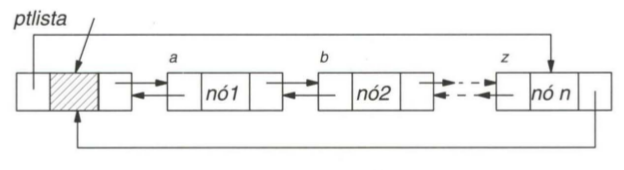
\includegraphics[width=.9\linewidth]{fig/listadoble.png}
\begin{itemize}
\item dois ponteiros: para o anterior e o posterior
\item percurso bidirecional
\item remoção necessita de um ponteiro
\end{itemize}
\section{Ordem Crescente}
\label{sec-3}
\subsection{Controlado no momento da inserção}
\label{sec-3-1}
\section{Vantagens e Desvantagens}
\label{sec-4}
\subsection{Vantagens e Desvantagens}
\label{sec-4-1}
\subsubsection{Lista Simples}
\label{sec-4-1-1}
\begin{itemize}
\item (+) menor custo de memória
\item (-) remoção necessita de dois ponteiros
\end{itemize}
\subsubsection{Lista Dupla}
\label{sec-4-1-2}
\begin{itemize}
\item (+) inserção imediata na última posição
\item (-) consome o \textbf{dobro} de memória para ponteiros
\end{itemize}
\subsection{Complexidade conhecida na literatura -- $\mathcal{O}(n)$}
\label{sec-4-2}
\begin{description}
\item[{Lista simples}] no pior caso, percorre a lista completa para inserir
\item[{Lista dupla}] no pior caso, percorre até o penúltimo nó
\end{description}
\section{Algoritmo}
\label{sec-5}
\begin{verbatim}
for (qtd = 1; qtd <= MAX; qtd *= 2) // mais pontos
  {
    // completa a lista
    for (i = 0; i < (qtd / 2); ++i)
      l=insercao_enc(rand() % MAX, l); //

    time(&inicio_conta);
    for (i = 1; i <= CANT_TESTE; ++i)
      {
        num = rand() % MAX;
        l=insercao_enc(num,l);
        l=remocion_enc(num,l);
      }
    time(&fim_conta);
    total = fim_conta - inicio_conta;
  }
\end{verbatim}
\section{Resultados}
\label{sec-6}
\subsection{Tabela com t vs n}
\label{sec-6-1}
\subsection{Gráfico t vs n}
\label{sec-6-2}
\section{Discussão dos resultados}
\label{sec-7}
\subsection{Esperado: O(n)}
\label{sec-7-1}
\subsection{Obtido: ??}
\label{sec-7-2}
\section{Bibliografia}
\label{sec-8}
\subsection{Livro da profa.}
\label{sec-8-1}
% Emacs 24.5.1 (Org mode 8.2.10)
\end{document}
